\documentclass{beamer}

\usepackage[utf8]{inputenc}
\usepackage{tipa, vowel}
\usepackage{textcomp}

\usetheme{metropolis}
%\usecolortheme{beaver}

\title[Project Presentation] %optional
{Finnish Phonotactics}

\subtitle{Presented by: Andrew Liu}

\setbeamertemplate{sections/subsections in toc}[square]

\author{Kaitlyn Du, Rocky Duong, Andrew Liu, Anton Than}

\date {5 October, 2022}

\begin{document}

\renewcommand\thefootnote{\relax}

\frame{\titlepage}

\begin{frame}
	\frametitle{References}
	We heavily used the Kari Suomi textbook, \emph{Finnish Sound Structure}, co-written with Juhani Toivanen and Riikka Ylitalo. Other authors' papers were used to confirm this information, including Arto Anttila, Thomas Berg, John Goldsmith, and Scott Myers.

	We also consulted with some Finnish speakers for this project. We communicated with a native Finnish speaker, Mette Laine for confirmation of some phonological information we found online. Lastly, many pronunciation guides came from a C1 Finnish learner, August Blackham.
\end{frame}

\begin{frame}
	\frametitle{Intro}
	{\large This presentation is based on the \textbf{Standard Finnish} dialect, spoken mostly in the Southern areas of Finland, and also used by professional speakers of Finnish.}
\end{frame}

\begin{frame}
\frametitle{Table of Contents}
\tableofcontents
\end{frame}

\section{Part 1 --- Phoneme inventory and phonotactics}

\subsection{Consonants}

\begin{frame}
	\frametitle{Consonant Inventory (Suomi et al, 2008, p 23.)}
	\begin{center}
	\scalebox{0.65}{
	\begin{tabular}{|l|c c|c c|c c | c c | c c| c c| c c| c c |}
		\hline
		& \multicolumn{2}{|c|}{Bilabial} & \multicolumn{2}{|c|}{Labiodental} & \multicolumn{2}{|c|}{Dental} & \multicolumn{2}{|c|}{Alveolar}  & \multicolumn{2}{|c|}{Postalveolar} & \multicolumn{2}{|c|}{Palatal} & \multicolumn{2}{|c|}{Velar} & \multicolumn{2}{|c|}{Glottal}\\\hline
		Plosive   & p & (b) & & & \multicolumn{3}{|r}{t} & \multicolumn{3}{l|}{\hspace*{.1in}d} & & & k & (g) & \textipa{(P)} & \\\hline
		Nasal     & & m & & & \multicolumn{3}{|r}{} & \multicolumn{3}{l|}{\hspace*{.1in}n} & & & & \textipa{N} & & \\\hline
		Trill     & & & & & \multicolumn{3}{|r}{} & \multicolumn{3}{l|}{\hspace*{.1in}r} & & & & & & \\\hline
		Fricative & & & f & \hspace*{.1in}v & & & s & & (\textipa{S}) & & & & & & h & \\\hline
		Approximant & & \textipa{V} & & & \multicolumn{3}{|r}{} & \multicolumn{3}{l|}{\hspace*{.1in}} & & j & & & & \\\hline
		Lat. Approx & & & & &  \multicolumn{3}{|r}{} & \multicolumn{3}{l|}{\hspace*{.1in}l}  & & & & & & \\\hline
	\end{tabular}
	}
	\end{center}
\end{frame}

\begin{frame}
	\frametitle{Notable Properties}
	\begin{itemize}
		\item Typically, /t/ is realized as \textipa{[\|[t]}, whereas /n/ and /d/ are alveolar
		\item Fricatives are rare, and typically only found natively in Southwestern dialects. /f/ is typically able to be distinguished, but /s/ vs. /\v{s}/ \textipa{[S]} is not. 
			\begin{itemize}
				\item Though, the example of \v{s}akki (chess) and sakki (a gang of people) is typically distinguished. (Laine, 2022)
				\item The orthography also includes /z/ and /\v{z}/, but is rarely used except for loan words.
			\end{itemize}
		\item The /d/ is also usually realized as a tap or flap \textipa{[R]} rather than the true plosive \textipa{[d]}. (Laine, 2022)
		\item The glottal stop is not in the orthography, but rather used to separate two adjacent vowels across syllable boundaries in a Sandhi phenomenon. (Suomi et al, 2008, p. 46.)
	\end{itemize}
\end{frame}

\begin{frame}
	\frametitle{Voiced plosives}
	\begin{itemize}
		\item /b/ and /g/ used to only be found in loaned words, but has made its way into Finnish orthography. (Laine, 2022)
			\begin{itemize}
				\item Some words that show these voiced plosives as minimal pairs to their unvoiced counterparts are \textipa{/gorillA/} (gorilla) and \textipa{/korillA/} (on a basket). (Laine, 2022)
			\end{itemize}
		\item In addition, /d/ is sometimes assimilated to \textipa{[t]}. (Laine, 2022.)
	\end{itemize}
\end{frame}

\subsection{Vowels}

\begin{frame}
	\frametitle{Vowel Inventory (Suomi et al, 2008, p. 20)}
	\begin{center}
		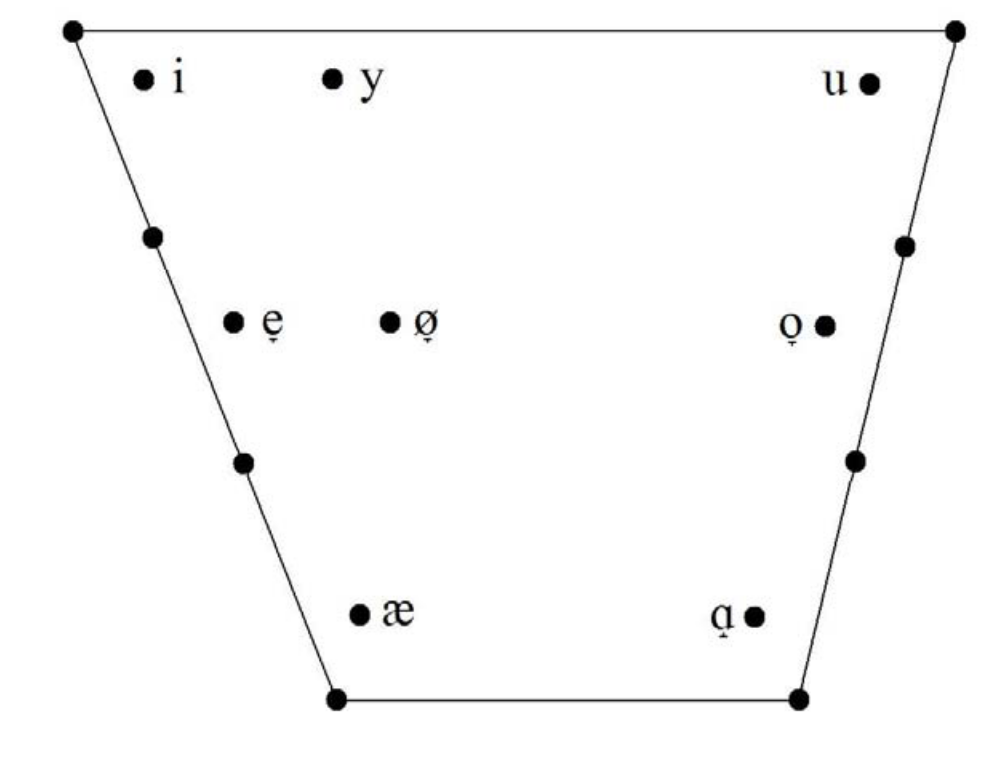
\includegraphics[width = .75\textwidth]{Images/vowels.png}
	\end{center}
\end{frame}

\begin{frame}
	\frametitle{Dipthongs (Suomi et al, 2008, p. 49)}
	\begin{center}
		\begin{tabular}{|c|c|c|c|c|}
			\hline
			 & /-\textipa{i}/ & /-\textipa{u}/ & /-\textipa{y}/ & Opening diphthongs \\\hline
			/\textipa{A}-/ & ai [\textipa{A\u*{i}}] & au [\textipa{A\u*{u}}]& & \\\hline
			/\textipa{\ae}-/ & \"ai [\textipa{\ae \u*{i}}]& & \"ay [\textipa{\ae \u*{y}}]& \\\hline
			/\textipa{o}-/ & oi [\textipa{o\u*{i}}]& ou  [\textipa{o\u*{u}}]& & \\\hline
			/\textipa{e}-/ & ei [\textipa{e\u*{i}}]& eu [\textipa{e\u*{u}}]& ey [\textipa{e\u*{y}}]& \\\hline
			/\textipa{\o}-/ & \"oi [\textipa{\o\u*{i}}] & \"oy [\textipa{\o\u*{y}}]& & \\\hline
			/\textipa{u}-/ & ui [\textipa{u\u*{i}}]& & & uo [\textipa{u\u*{o}}]\\\hline
			/\textipa{i}-/ & &  iu [\textipa{i\u*{u}}]& iy [\textipa{i\u*{y}}]& ie [\textipa{i\u*{e}}]\\\hline
			/\textipa{y}-/ & yi [\textipa{y\u*{i}}]& & & y\"o [\textipa{y\u*{\o}}]\\\hline
		\end{tabular}
	\end{center}
\end{frame}

\begin{frame}
	\frametitle{Notable Properties}
	\begin{itemize}
		\item Nasalization (Laine, 2022)
			\begin{itemize}
				\item Finnish vowels undergo nasalisation in the vicinity of nasal consonants.
			\end{itemize}
		\item Vowel Harmony (Laine, 2022)
			\begin{itemize}
				\item In Finnish, the back vowels a, o and u only appear with each other and e, i.
				\item Likewise, the front vowels \"a, \"o and y only appear with each other and e, i 
				\item These rules apply to most non-compound, non-loaned words.
			\end{itemize}
		\item Doubled vowels (Suomi et al, 2008, p. 22)
			\begin{itemize}
				\item In Finnish, doubled vowels (e.g. \"o\"o vs. \"o) are minimal pairs.
				\item E.g. \emph{tuuli} (wind) vs. \emph{tulli} (customs at a border crossing)
			\end{itemize}
	\end{itemize}
\end{frame}

\subsection{Phonotactics}

\begin{frame}
	\frametitle{Phonotactics (Suomi et al, 2008, pp 49--61.)}
	\begin{center}
		\fbox{
			\begin{minipage}{3.5in}
		The general syllable structure is CVC, with occasional doubled vowels, and doubled consonants mostly from loaned words.
			\end{minipage}
		}
	\end{center}
	
\end{frame}

\begin{frame}
	\frametitle{Phonotactics (Suomi et al, 2008, pp 49--61.)}
	\begin{itemize}
		\item Vowels
		\begin{itemize}
			\item All vowels can occur doubled, and there are 18 dipthongs. In addition, sequences of 3--4 vowels can occur, which come from shorter subsequences of vowels and/or dipthongs.
			\item Vowel harmony
		\end{itemize}
	\item Consonants
		\begin{itemize}
			\item \textipa{/ p \|[t k s h l r m n j V d f b g S /} all occur word initially.
			\item Additionally, \textipa{/ pl pr \|[tr kl kr/} are plosive + liquid sequences that can occur word initially, as do \textipa{/ sp sk s\|[t /}. Very rarely, word initial CCC sequences can occur: \textipa{/ spr s\|[tr /}
			\item Word internally, all C sequences, except \textipa{/N/} can occur
		\end{itemize}
	\end{itemize}
\end{frame}

\begin{frame}
	\frametitle{Phonotactics --- Consonant Sequences (Suomi et al, 2008, pp. 55--58.)}
	\begin{itemize}
		\item Doubled consonants can occur at syllable boundaries.
		\item There are some other rules that are usually only violated in the case of loan words:
			\begin{itemize}
				\item A nasal cannot follow a plosive
				\item /l/ and /s/ cannot be followed by /r/
				\item A liquid cannot follow a nasal
				\item A consonant cannot follow a central approximant
				\item /h/ cannot follow an obstruent
				\item A central approximant cannot follow plosives other than \textipa{/\|[t/}
				\item A  heterorganic consonant cannot follow a nasal
				\item A labial plosive cannot be followed by a non-labial plosive, and vice versa
				\item A dentialveolar plosive cannot follow a velar plosive.
			\end{itemize}
	\end{itemize}
\end{frame}

\begin{frame}
	\frametitle{Phonotactics cont. (Suomi et al, 2008, pp 58--61.)}
	\begin{itemize}
		\item CCC sequences --- word-internal
			\begin{itemize}
				\item In word-internal CCC sequences, there is always a syllable boundary before the last consonant.
			\end{itemize}
		\item Word-final consonants
			\begin{itemize}
				\item In native words, only \textipa{/\|t/}, /s/, /n/, /l/, and /r/ occur word finally.
				\item In loaned words, many attempts are made to avoid ending consonants by adding a vowel to the end, much like Spanish's leading vowels for loan words.
			\end{itemize}
		\item More rules
			\begin{itemize}
				\item \#CV restrictions: /ji/, /je/, \textipa{/Vu/} are prohibited.
				\item \#VV restrictions: /ii/, /ie/, /uo/ are prohibited / rare.
				\item \#(C)VVCC restrictions: complicated.
			\end{itemize}
	\end{itemize}
\end{frame}

\section{Part 2 --- Phonological Processes}

\subsection{Conditioning of Central Approximants}

\begin{frame}
	\frametitle{Conditioning of Central Approximants}
	In Finnish, these sounds occur in syllable onsets, and the phoneme /v/ has two allophones: (Suomi et al, 2008, p. 31)
	\[
		/\text{v}/ \rightarrow
		\begin{cases}
			[\text{\textipa{w}}] & / \text{ after diphthongs ending in u}\\
			[\text{\textipa{V}}] & / \text{ elsewhere}\\
		\end{cases}
	\]
	These are demonstrated in the below words/phrases:
	\[
		\text{\emph{sauva} \textipa{[sAuwA]}} \qquad \text{\emph{rouva} \textipa{[rouwA]}}
	.\]
	
\end{frame}

\subsection{Allophones of /h/}

\begin{frame}
	\frametitle{Allophones of /h/}
	In Finnish, the letter h appears in syllable and word final and initial positions. Consider some pronunciations of the following words (Suomi et al, 2008, p 28).
	\begin{columns}
		\begin{column}{.45\textwidth}
			\begin{center}
				\begin{tabular}{c c}
					\emph{vihma}& \textipa{[vi\c{c}mA]}\\
					\emph{pihvi} & \textipa{[pi\c{c}vi]}\\
					\emph{lyhty} & \textipa{[l\super wy\c{c}\|[ty]}\\
					\emph{vihje} & \textipa{[vi\c{c}j\|`e]}\\
					\emph{vihko} & \textipa{[vi\c{c}k\super w\|`o]}\\
					\emph{tahma} & \textipa{[taxmA]}\\
					\emph{kahvi} & \textipa{[kaxVi]}\\
					\emph{tuhti} & \textipa{[\|[tux\|[ti]}\\
				\end{tabular}
			\end{center}
		\end{column}
		\begin{column}{.45\textwidth}
			\begin{center}
				\begin{tabular}{c c}
					\emph{kohme} & \textipa{[koxme]} \\
					\emph{tuhka} & \textipa{[\|[tuxkA]}\\
					\emph{vihi} & \textipa{[ViHi]}\\
					\emph{v\"ah\"a} & \textipa{[V\ae H\ae]}\\
					\emph{vaha} & \textipa{[VAHA]}\\
					\emph{haamu} & \textipa{[hA:mu]}\\
					\emph{t\"ahti} & \textipa{[\|[t\ae h\|[ti]}\\
					\emph{lehv\"a} & \textipa{[lehv\ae]} 
				\end{tabular}
			\end{center}
		\end{column}
	\end{columns}
\end{frame}

\begin{frame}
	\frametitle{Allophones of /h/}
	Based on the above, the following rule was proposed by Suomi et. al, on page 28:
	\[
		/\text{h}/ \rightarrow
		\begin{cases}
			[\text{\textipa{\c{c}}}] & / \text{ between a high front vowel and a consonant}\\
			[\text{\textipa{x}}] & / \text{ between a back vowel and a consonant}\\
			[\text{\textipa{H}}] & / \text{ between vowels, especially word-internally}\\
			[\text{\textipa{h}}] & / \text{ elsewhere}\\
		\end{cases}
	\]
	Note that the fricative allophones \textipa{[\c{c}]} and \textipa{[x]} occur syllable finally, while the glottal allophones occur syllable initially. (Suomi et al, 2008, p. 28)
\end{frame}


\section{Sources}

\begin{frame}
	\frametitle{Citations}
	\setbeamertemplate{bibliography item}[text]
	\begin{thebibliography}{10}
		\bibitem{antilla} Anttila, A. (2001). Variation in Finnish phonology and morphology - universiteit van amsterdam. Retrieved October 2, 2022, from https://fon.hum.uva.nl/paul/papers/reviewAnttila\_glot2001.pdf 
		\bibitem{thingy} BERG, T., \& KOOPS, C. (2015). Phonotactic constraints and sub-syllabic structure: A difficult relationship. Journal of Linguistics, 51(1), 3--39. http://www.jstor.org/stable/24583228
		\bibitem{goldsmith} Goldsmith, J. (1985). Vowel Harmony in Khalkha Mongolian, Yaka, Finnish and Hungarian. Phonology Yearbook, 2, 253--275. http://www.jstor.org/stable/4419959
	\end{thebibliography}
\end{frame}

\begin{frame}
	\frametitle{Citations}
	\setbeamertemplate{bibliography item}[text]
	\begin{thebibliography}{10}
		\bibitem[4]{meyers} Myers, S., \& Hansen, B. B. (2007). The Origin of Vowel Length Neutralization in Final Position: Evidence from Finnish speakers. Natural Language \& Linguistic Theory, 25(1), 157 -- 193. http://www.jstor.org/stable/27642859
		\bibitem[5]{goat} Suomi, K., Toivanen, J., Ylitalo, R. (2008). Finnish sound structure: Phonetics, phonology, phonotactics and Prosody. University of Oulu. 
	\end{thebibliography}
\end{frame}

\begin{frame}
	\frametitle{Citations --- People}
	\setbeamertemplate{bibliography item}[text]
	\begin{thebibliography}{2}
		\bibitem{Blackham} Blackham, August, Personal Communication. (October 1, 2022).
		\bibitem{Laine} Laine, Mette, Personal Communication. (October 1, 2022).
	\end{thebibliography}
\end{frame}

\end{document}
